\chapter{Introduction}
\label{ch:introduction}
\graphicspath{{chapters/00_introduction/figures/}}

% \dictum[Immanuel Kant]{%
%   Sapere aude! Habe Mut, dich deines eigenen Verstandes zu bedienen! }%
% \vskip 1em

% \begin{otherlanguage}{ngerman}
% Die ältesten Bestimmungen der wahren Grösse der Moleküle hat die kinetische
% Theorie der Gase ermöglicht, während die an Flüssigkeiten beobachteten
% physikalischen Phänomene bis jetzt zur Bestimmung der Molekülgrössen nicht
% gedient haben. \dots
% \end{otherlanguage}

\section{Prologue: Motivation\textsuperscript{*}} %Prob rename it as Preamble
\footnotetext{* A version of this prologue has been published as part of the book chapter: \fullcite{ArgotaSanchez-Vaquerizo2023_3Tales}}

We approach our cities in contradictory ways. On one hand, we aim to control, predict, and design them top-down \citep{Gaffron2005}. On the other hand, cities are complex entities \citep{Port00} in constant change whose functioning is extremely hard to grasp. This means that they are ill-suited to traditional control approaches. Problems and conditions are always evolving with every single change or after a solution is provided. Understanding the manifold interactions between the built environment and its inhabitants requires powerful tools \citep{Fink2018} beyond traditional practice and purely human skills.

Digital abundance \citep{Hovestadt2017} enables the most recent iteration of incorporating computational tools for city-making: smart cities. However, their promise of hyperefficient management of cities \citep{Picon2015} falls short \citep{Greenfield2013}. They are mostly disconnected, \emph{ad hoc}, utilitarian, and technical single-dimension optimization processes \citep{Wilson2018} with very limited impact on the expected overall quality of life in our environment \citep{Batty2020smartcities}. They focus mainly on the ‘high-frequency’ city. It is, changes we experience in real-time, at the scale of seconds, minutes, days and months \citep{Batty2018AIandSmartCities, Wildfire2018}, while disregarding longer-term planning. Simultaneously, the abundance of data and digital resources enhances participation and commoning processes \citep{Cardullo2019, Mainka2016} that counterbalance top-down and technocratic visions for the production of cities \citep{Lefebvre1974}. But such a counterbalance cannot be taken for granted, as unbalanced power and information-sharing capabilities among parties may hinder the quality of this participation \citep{Pateman1970}.

Underlying both approaches is the inherent difficulty of grasping and measuring the components of urban life \citep{DeNadai2016}: from geometric and physical features of space to interactions and cognitive processes that are hard to quantify, as is the case with the qualitative aspects of any human-related system \citep{Helbing2021}.

This situation suggests a need to reformulate the role and scope of city planning \citep{Cuthbert2006, Ratti2015}, as already anticipated by more open-ended dynamic, systemic, and participatory approaches such as those embedded within planning support systems (PSS) \citep{Geertman2020}. In contrast to the postulates of the end-of-history \citep{Fukuyama1992} and end-of-science \citep{Anderson2008,Carpo2014}, which assume the steadiness of our world in combination with some sort of technological determinism \citep{Lanier2013}, the constant changes in our environmental conditions require permanent revision and adaptation. Crises cause our planned cities to come apart at the seams. Rigid functional planning proves to be segregating and detrimental to cities and leaves little room for change and adaptation \citep{Jacobs1961, Mantysalo2005, Verebes2014}. Unsurprisingly, this shortcoming permeates everywhere in the built environment: homes are too inflexibly designed to cope with the changing needs of their dwellers, and streets are forced to cope with peak hour traffic while hindering any alternative or unplanned uses \citep{Bereitschaft2020, Southworth1997}. We barely give a chance to people to determine their own preferences and use these preferences for the benefit of spatial planning. Hence, we need to find ways of embedding adaptability and resilience in city-making processes by design. 

Therefore, this text introduces three visions of how future policy and decision-making for city co-creation could use comprehensive urban simulations. More than for their predictive, deterministic power, in these visions, urban digital twins \citep{Batty2018AIandSmartCities} are valuable because they enhance the collaborative exploration of ‘what-if’ scenarios \citep{Dembski2020} that could inform more resilient and adaptable cities through unbounded multiobjective optimization \citep{Deb2014}. This means identifying alternatives that effectively consider several goals simultaneously. At different scales, components, and cycles \citep{Gaffron2005}, three future cities are described where computational approaches and machine intelligence are merged with human preferences and skills to articulate new strategies of urban planning able to cope with the complex interplay of stakeholders’ agencies involved \citep{Quan2019} in an unpredictable and changing world. This means, altogether, more informed, more diverse, more uncertain, and more flexible cities existing after our time.

\setcounter{figure}{-1}
\begin{figure}[htbp!]
    \centering
    \includegraphics[width=1\textwidth]{chapters/00_introduction/figures/fig_01_the_city_is_result_r.jpg}
    \captionsetup{format=plain, justification=centering} % Center the caption
    \caption{The city is result of the active, collaborative, and co-learning process between \textcolor{red}{physical} and \textcolor{green}{virtual} agents}
   \label{fig:gree_red}
\end{figure}
\FloatBarrier

% \section{Objectives / Research questions}
% Cities are among the most complex human creations \citep{Portugali}. They are result of bottom-up and top-down processes, exhibit emergent features, are in permanent transformation and feature non-stationary problems \citep{Gershenson2013}. They are simultaneously (self-)organized and chaotic. Therefore, cities are not suitable for conventional control approaches. Contrary to the contemporary, modernist, and mechanistic conception of urban planning where everything in the city can be masterplanned, the conditions and dynamics of the city are always evolving, endlessly escaping planners' minds, always one step ahead: every time an intervention or solution is proposed, the whole set of conditions will change, making it immediately outdated.

% Urban complexity involves also the interplay of human behaviour.
% % check presentation
% Understanding this complex interplay of the built environment and people behaviour requires powerful tools \citep{Fink} that are able to expand human cognition and skills. Statistics, machine learning, data science, simulation, complex science, and artificial intelligence can come into play to provide support in decision-making and urban planning for cities, within multidisplinary team, including experts and no-experts, combining different agendas, and making sense of diverse crowd-sourced knowledge \citep{participationUrban} \citep{Surowiecki2005}.

%%
%%
\section{Research overview}

This thesis has been developed as part of the ERC-funded project Co-Evolving City Life (CoCi) project (grant agreement No. 833168 ). CoCi aims to research new concepts for more resilient, sustainable, and participatory cities. Particularly, the thesis expands on two of the work packages of the project (Figure~\ref{fig:inception}):
\begin{itemize}
    \item \textbf{WP1:} More resilient cities. Digitally assisted cooperation.
    \item \textbf{WP2:} Self-organizing cities. Co-learning. 
\end{itemize}

The thesis illustrates how urban modeling and simulation can be utilized for city planning and policy-making. The research provides insights that challenge current decision-making processes, including participatory ones, and common assumptions in planning and design. By examining three case studies at different spatial urban scales, it addresses three different significant and actual challenges faced by cities, using different cutting-edge methods and techniques to provide new perspectives that can aid in future city-making processes:
\begin{itemize}
    \item Small spatial scale ($<10^2 m$) on adaptive street design, and human-traffic interaction using virtual reality (VR).
    \item Medium spatial scale ($10^2 - 10^3 m$) on detecting counterintuitive positive effects on traffic from road network reduction using microscopic agent-based modeling.
    \item Large spatial scale ($>10^3 m$) on land use changes from adaptive reuse of offices into housing and how it affects traffic demand using spatial econometrics models. 
\end{itemize}

\begin{figure}[htbp!]
    \centering
    \includegraphics[width=1\textwidth]{chapters/00_introduction/figures/inception_01_v01.jpg}
    \captionsetup{format=plain, justification=centering} % Center the caption
    \caption{General research framework and connection with Co-evolving City Life (CoCi) project. The thesis considers three spatial scales in four chapters, and it participates of two work packages of the CoCi project.}
   \label{fig:inception}
\end{figure}

%% It is about Barcelona. Why Barcelona?
These three case studies are examples of the complex, unexpected, and non-intuitive behavior of urban systems. Therefore, they aim to show technical implementations of urban simulations that can be integrated into current decision-making and planning for cities. They are designed to provide support for non-experts and experts and to shed light on the, sometimes unexpected and counterintuitive, impact of their opinions and decisions. Thereby, the methods presented in this thesis can be a resource to learn and tune planning and policy-making processes as illustrated by the results. 
 
The research presented in this thesis shows an interest in better, more sustainable, and resilient cities. It aims at overcoming utilitarian single-dimensional optimization processes focusing on individual and isolated aspects of urban life, frequently connected to the \emph{high-frequency} city. However, the longer-term, \emph{low-frequency} city is crucial for planning \citep{Batty2020smartcities}.
%multi-objective optimization % check p[roposal]
% participation
% uncertainty quantification associated to socio-technical human systems
The built environment is core to the thesis, and hence it is situated. For the medium and large scale, the thesis uses real data, policies and issues found in Barcelona, Spain. Nonetheless, they are extrapolable to many other cities around the wold, as they are some of the ideas and policies originated in Barcelona. The small scale, although inspired by real locations, could be any street around the globe.

The three case studies focus on how people move and interact at these different scales across the city. By being closer to the social-human aspects of cities, the thesis challenges technocratic visions of urban models and related doubles which frequently overrepresent physical assets, and hence, it acknowledges the need for improving our understanding and foster efforts to represent socio-economic aspects of cities, that involve human, social, cultural and psychological factors \citep{Batty2018}. This means also embracing the uncertainty intrinsic of such socio-technical human-related complex environments \citep{Caldarelli2023} that may render extremely complicated, if not unfeasible, their predictability \citep{Cureton2020}.
Thereby, this thesis pinpoints how the value of these models and simulations is not in their predictive power \emph{per se} to forecast deterministically and undoubtedly the future of cities. Differently, these systems are more valuable for their exploratory power, for shaping thinking and helping us to pose questions \citep{Kac1969}. 
% It is, directly connected to the role of architecture, design and planning 
At a higher level, the thesis presents computational approaches that enhance human cognition and configure a hybrid intelligence able to tackle urban challenges with more complete, complex, and effective knowledge.
In broader terms, this research proposal follows the interest of reconciling structuralist quantitative and positivist approaches of city and regional science with the humanistic-phenomenological qualitative and hermeneutic social theory of cities \citep{Port00}.

\subsection{Modelling and quantitative perspectives in city-making}

Quantitative approaches towards the study and understanding of cities and the use of modeling and simulation as a way of inquiring about the potential impacts of our decision-making in the future of our built environment articulate the backbone of the thesis. Therefore, this subsection offers a general overview of different approaches towards simulation and modeling applied to urban policymaking, design, and planning which are transversal to the entire thesis. As such, it helps to anchor the presented research in the historical literature that has approached urban complexity from quantitative and computational methods. At the same time, it connects with urban theory and cognitive science to better understand how people construct, perceive, and are affected by the built environment. Each chapter provides a more detailed literature review and context directly connected to the urban issues, topics, and methods used for each urban scale.

Transportation is a fundamental aspect of the rise of urbanism as a discipline \citep{Cerda1867} in parallel with the development of the industrial city \citep{CIAM1933}. However, urban planning and design encompass more than just transportation, and the resulting city is the consequence of feasible compromises among various stakeholders and their agendas \citep{Zografos2020}. Cities are often seen as ``wicked" problems \citep{Rittel1973}, and the lack of empirical support undermines informed and effective decision-making, evaluation, and iterative improvement processes for technical specialists, officials, and citizens. The complexity of urban systems has been reflected in qualitative urban studies and theory \citep{Lynch1960, Jacobs1961, Christopher1965}. While early attempts at quantitative urbanism showed a clear interest in how people used and experienced the space \citep{Whyte1979, Ewing2013}, these quantitative approaches applied to urban form have been more focused on land use \citep{Parker2003, White2015}, mobility \citep{Barbosa2018HumanApplications}, city fabrics and transportation networks \citep{Boeing2019UrbanSpatialOrder,Xie2009,Zanin2018}, and in general large-scale, complex features of human settlements \citep{Batty2008CitiesComplexSys, Bettencourt2007, Schlapfer2015, Schlapfer2020}. Space Syntax \citep{Hillier1984} stands out among the graph-related applications due to its wide and steady use and long development in trying to relate quantification of the complexity of the built environment with people's perception and quality of life. This connects to recent advancements in updating research and practice of spatial planning and design which recover the interest in understanding the complex interactions happening between the built environment and human cognition of space \citep{Piaget1948, Li2016, Arnheim1954, Derix2013, Dubey2023}.
More recently, the popularization of the Sustainable Development Goals (SDG) involves the use of concrete indicators covering a myriad the aspect of urban life, whose evaluation requires the challenging  development of clear quantification standard across the world \citep{Mair2018,Tzachor2022}.  
%% Urban analytics, and how it connects to quantifiable urban factors: SDG and VNR and VLR.

Computer simulations have long been used in spatial and transportation planning. Land use-transportation interaction (LUTI), econometric, and urban economic models \citep{Echenique2004EconometricTransportation}, emerged in the 1950s to predict the outcome of policy and urban planning decisions \citep{Lowry1964, Forrester1969}, when cities were conceptualized as optimization problems linked to defense-related agendas and transportation modeling \citep{HousingAct1949, HighwayAct1956, UrbanMassTranspAct1964, Kristof1972, Weiner2013}, echoing cybernetic and control theory frameworks \citep{CardosoLlach2015, Pask1969, Pask An Approach to Cybernetics, Wiener194x}. These early models, despite gaining sophistication by incorporating behavioral theories like bid-rent \citep{Alonso1964LocationRent} and discrete choice \citep{McFadden1978}, faced criticism for their unreliability and high requirements \citep{Lee1973RequiemModels}. The slowing down and lack of enthusiasm didn't avoid the further development and proliferation of different LUTI models until nowadays \citep{Southworth1995, Iacono2008, Waddell2002Urbansim:Planning, Wegener2021Land-UseModels, Hunt2005, Timmermans2003, Acheampong2015, Thomas2018CityDeliLUTI, Lopes2019LUTI, Moeckel2018}. As a result, we can differentiate two big families of models: (1) equilibrium-based theoretical dynamic models, and (2) bottom-up land-development models based on the aggregation of spatial units (i.e. cellular automata --CA-- models) or individual actors (agent-based models--ABM) \citep{Heppenstall2012}. The exponential growth of computation capabilities has particularly bolstered the development of these bottom-up models, allowing for an increasing consideration of finely disaggregated urban phenomena at very small detail (e.g. microsimulation) adding incremental dynamic to traditionally static large models \citep{Batty2013SIMULACRA,GarciaCantuRos2014,Cottineau2015}.

Urban modeling found in transportation one of the most fertile fields, utilizing simulation as a dynamic partial computational representation of the real world \citep{Drew1968} to optimize infrastructure design in practice \citep{HCM2016}. One of the main advantages of these many-particle simulations is making understandable and explainable the complexity of traffic and mobility patterns \citep{Helbing2001Many}. Furthermore, bottom-up approaches in modeling, as in ABM, allow for simulating individual human behavior, following the assumption that cities emerge from the aggregation and interactions of individual actions. Despite the limited understanding of how individual actions are connected to spatial features and urban systems, the resource abundance \citep{Hovestadt2017, Carpo2014} of computational, sensing, and data resources can help to develop, test and tune new theories bridging individual behavior, the built environment and modeling across different spatio-temporal scales \citep{Heppenstall2016}. However, this approach does not mean to endorse the idea of the "end of theory" \citep{Anderson2008}, but rather the opposite: to create highly accurate, interactive digital mirrored representations of real physical and functional processes of socio-economic systems in cities, and coupled in near real-time \citep{Batty2018, Mathias2020, Lei2023, Jeddoub2023}.

Disaggregated, bottom-up models are very suitable for simulating and studying cognitive processes at the individual level regarding how people move and relate to space, such as wayfinding, object placement in retail, emergency and evacuation scenarios, and in general self-organized crowd-behavior \citep{Timmermans2009}. However, the complex entire cognitive process when people move and interact in space is an active field of research \citep{Dubey2018TowardsEnv,Dubey2019FusionSources}. These frameworks can help in increasingly complex urban environments, with new dynamic and fast-paced interactions and new layers of information, as in the case of new autonomous vehicles and other smart solutions for transportation and mobility management \citep{Duarte2018,Dubey2024AdapLanes,Dubey2024Fairlane}. Interaction between autonomous vehicles and pedestrians has received most of the attention \citep{Jayaraman2019}, however, it is unknown, and it is subject to current research and policy and design practice to determine how these new technologies will reshape urban spaces and challenge our existing street paradigms \citep{ Meyboom2018,Riggs2020}.    
Computer simulations are increasingly gaining adoption for unraveling urban life's many components and hence, for informing policy and planning making \citep{Batty2005Agents}. They support current planning practices that integrate, among others, adaptive reuse and inner city renovation, environmental concerns, intense use of sensing, data and analytics, new mobility options, and citizen engagement. As a result, models are used more frequently to simulate current and future scenarios \citep{Guzman2014,Wang2015, Batty2020} or even to drive new urban developments from scratch. In this sense, part of these trends converges with the broad category of smart cities \citep{Batty2020smartcities}, and more recently is expanded in the so-called urban digital twins.
In this sense, the implementations illustrated in the thesis approach cities from a quantitative point of view, to tackle socio-technical challenges relevant to public --and political-- debate, that concerns people's experiences and behavior in the city. 
%This thesis contributes to planning support research by developing new methods for co-creating cities using modeling tools, public participation, and AI/ML techniques, aiming for multi-objective planning at various scales.

%This growing value of simulations is enhanced by their integration into larger frameworks for supporting planning (PSS or Planning Support Systems). From their origins deeply rooted into early management science’s decision support systems (DDS), they evolved to be communicative tools to design with people [23], [107]. In the process they were enriched by more data, spatial capabilities, better interfaces, tools for generating solutions, models, and participatory open-ended processes inspired by novel ideas such as geodesign [108] Precisely, this thesis aims to contribute to the research on planning support research by providing new methods of co-creating cities combining modeling tools and people’s participation with the assistance of artificial intelligence and machine learning techniques.


\subsection{Expanding Urban Digital Twins as socio-technical tools for city-making}

The implementations presented in this thesis elaborate and expand on the subject of urban digital twins \citep{Batty2018, Ferre-Bigorra2022TheTwins}. Inspired by the original concept of digital twins from the manufacturing and aerospatial industry \citep{Grieves2014, Shafto2012}, the idea of creating very realistic, accurate, and interactive near real-time digital representations of cities has been gaining popularity in recent years. However, the own definition of urban digital twin is ambiguous and lacks clarity. In fact, this term is used to name different implementations of similar ideas \citep{Depretre2022, Shahat2021}. Recent reviews on the topic of urban digital twins simultaneously assess the very early stage of research on this topic and the many technical and non-technical challenges that urban digital twins face. Among these challenges, we can highlight the lack of definition and purpose, which is closely related to the lack of value, business model, and eventually support for their further development. 

The greater significance of technical challenges highlights the preference for technology-driven development in urban digital twins. This approach is arguably inherited from corporate technocratic methods used in smart cities \citep{Cardullo2019}, where optimization is the primary motivation \citep{Kitchin2016}. However, this approach dismisses socio-technical approaches that question this status quo based on data universalism \citep{Loukissas2019}, precisely to reveal pluralistic visions, phenomena, and experiences of cities \citep{Charitonidou2022}. 
Also, this highlights the contradiction caused by a pure technocratic vision as the construction of urban digital twins is expected to be the result of interdisciplinary collaboration between different domains, expertise, and stakeholders while simultaneously collecting the diversity of visions and interests in the built environment at a local level.
As a result, the current implementation of so-called urban digital twins is far from a full realization both as purely technical systems regarding standardization, interoperability, and scalability \citep{Cheng2022, Shahat2021} and as socio-technical construct regarding community participation \citep{Axelsson2018}.

%to discussion? 
This pluralistic and diverse understanding of the city also questions the mechanistic, lineal, and top-down master planning of the built environment that has dominated city-making during the last centuries \citep{Verebes2014}. Nevertheless, we can construct an approximation to an open-ended and ideal definition of urban digital twins as systems that coordinate and merge 3D realistic models of the built environment which include geometric and semantic information at different spatial and temporal scales, which are able to exchange and provide near real-time interactive data, and that as results enable multiple operations and address social and economic functions in the built environment \citep{Lei2023,Jeddoub2023}.

It is in this context where a stronger awareness of the social aspects of urban digital twins to design them with a human-centric perspective in mind \cite{Helbing2021}, focusing on people's concerns and making them as transparent, understandable, accountable, and operationalizable as possible, which involves fostering participation at its very basis \citep{White2021}. 

These concerns contextualize the work of the thesis on disciplinary, technical, and social dimensions.
% Pluralistic/plurality
% how does it relate to Urban DTs?
% \section{Research objectives}
Following these considerations, this thesis at a high level interrogates design practice in general, and in particular in the context of urban planning and architecture in cities with three overarching, nested, research questions:

% making easier and transparent models to use

\begin{itemize}
    \item From a disciplinary and professional perspective, what is the role of experts, technical staff, and practitioners (i.e. namely urban planners, architects, urban designers, and policymakers)?
    \item From a technical and operational perspective, how can we anticipate the outcomes of our decisions and plans for cities and integrate that learning in our processes (i.e. testing cities before they are "built")?
    \item From a social perspective, how can this help to coordinate and effectively articulate the complex interplay of stakeholders' agencies involved in city-making (e.g. designers and planners, engineers, computer scientists, policymakers, government agencies, and particularly citizens)? % check presentations who makes the city
\end{itemize}

While different, these three applications at different scales share their aim of addressing technical, disciplinary, and social questions by creating frameworks that can enhance human cognition with machine intelligence \citep{Licklider1960}, in a hybrid setting, with a two-fold goal:
\begin{itemize}
    \item Facilitating informed decision-making for citizens regarding city-making making accessible, understandable, and conceivable complex effects in urban systems.
    \item Enriching machine intelligence from human experience through machine-learning collaboration \citep{Licklider1960}.
\end{itemize}

% maybe dropping this 
%%%%%%
% TO DO: connecting the three scales in a simple tale
%%%%%%
% Therefore, for example, the spatial affordance \citep{affordance} of streets is determined by the design at a very small scale, and by the interactions of their users whose presence in the space is determined by the layout and distribution of activities and land uses of the city at larger scales. These flows surge as a result of a bottom-up self-organizing process. Simultaneously, the large-scale spatial patterns are not independent of individual decisions at a micro-level which are conditioned by rules and preexisting conditions operating at different scales. Nonetheless, changes at every level of instance will create a cascading effect propagating through the entire urban system in not necessarily predictable ways. Pedestrianizing a street may foster local business but disincentivizing the use of private vehicles  

Therefore the thesis aims at having a multi-scalar character, where each of the applications and domains at different scales covered in the chapters are interrelated subsystems of the urban system \citep{Batty2013}. An effective design of the city requires a holistic consideration across all its connected temporal and spatial scales, components, constituents, and cycles \citep{Gaffron2005}. 

\subsection{Positive counterintuitive and paradoxical effects in cities}
% on chasing counterintuitive effects
One common theme across all three case studies and their scales is the uncovering of counterintuitive effects of planning decisions. These insights, made possible by the use of urban simulation, illustrate how computational techniques can expand human cognitive capabilities. Our decision-making is bounded by knowledge, biological limits and influenced by biases. Thereby, the complexity of the built environment and urban systems often challenges our intuitive understanding of impacts, interactions, side, and cascading effects, even with supposedly well-informed decisions. Therefore, across various scales and methods addressing concrete urban issues, the case studies included in this thesis, reveal the unexpected positive impacts of certain policies, challenging many of the common assumptions, intuitions, and beliefs of both citizens and experts. 

% The uncovering of counterintuitive effects of planning decisions is another of the common threads linking all the scales and projects. This is a direct consequence of the use of urban simulation and a clear example of the expansion of human cognition enabled by computational techniques. Our decision-making is bounded by our knowledge and conditioned by our biases. However, the complex nature of urban settings escapes our intuition regarding the impacts, side, and cascading effects of our decision-making, even when it is supposed to be well-informed. At different scales, with different methods, and focusing on different urban topics, all the examples collected in this thesis show this discovery of positive effects of some policies which could be seen as opposed to common ideas, prejudgements, and intuitions in citizens and also, experts. 

In Chapter~\ref{ch:VR}, with a focus on a small spatial scale, the results of the  VR experiments on citizens' perception of adaptive street designs indicate that citizens do not immediately perceive the practical, utilitarian, and functional advantages facilitated by innovative adaptive design despite the increased flexibility, and how this acceptance is affected more by how communication of new projects is designed more than the tangible features and improvements. Even more clearly, Chapters~\ref{ch:getting_real} and \ref{ch:less_can_be_more} model at a medium spatial scale the effects of street closures and traffic calming related to Braess and Daganzo paradoxes \citep{Braess1969,Sheffi1978}. Using the example of the \emph{Superblocks} \citep{Rueda2018}, the models are able to positively exploit these paradoxes by identifying scenarios where a reduction of space for vehicles can have positive effects by reducing congestion and pollution. In a similar way, Chapter~\ref{ch:ETRCO2H} a large scale, modeling the impact that adaptive reuse and transformation of offices into housing \citep{Remy2014, Pratiwi2023}, and the consequent densification of the inner part of the city, does not necessarily cause an increase in traffic.

Altogether, the result of this work questions the common intuition that permeates public debate on urban issues. Hence, it pinpoints the value of these tools to inform and enrich city-making processes.

% simulation vs modeling
% unveiling complexities and unexpected conditions and effects that escape our human cognition


% NOTE: SDGs and VLRs. Dev of concrete metrics. % to discussion?

\subsection{Specific research topics}
%% summary of three scales
For each case study in a different urban scale, the thesis proposes a similar research framework, combining technical and applied (i.e. societal and policy) aspects. From a policy point of view, each application at a different scale focuses on a relevant urban issue that creates controversy in the current public debate, and which is directly connected to complex interactions and effects hard to predict. Hence, each of these blocks formulates a research question and hypothesis that somehow challenges existing common ideas on the topic of interest. In parallel, this question is responded also from a technical point of view, and further developed by a relevant technical research question that involves different data collection approaches and methodological innovations.

The small scale presented in Chapter~\ref{ch:VR} focuses on people's interactions with the immediate built environment, hence the suggested range of distance between $10^1$ and $10^2 m$. This block of the thesis uses VR experiments to interrogate how pedestrians would be impacted by innovative adaptable street designs and how communication of these new policies matters affects their acceptance. Traditional street design is static, segregates different flows, and tends to prioritize the traffic demand during peak hours. This hinders other users' needs for space and limits alternative activities in the limited public space in cities even when that space is not needed off-peaks. Currently, there are intense public debates about redistribution of the limited space of streets in cities and retrofitting urban design approaches from the past that prioritized motor vehicle traffic \citep{Norton2008}. New practices in urban planning nowadays aim to promote active and sustainable mobility and new advancements in autonomous driving and other technologies applied to traffic management and urban design can potentially support new flexible and dynamic approaches to mobility and urban challenges in the limited space of cities \citep{HamiltonBaillieEnv2008}. VR makes it possible to simulate in an immersive way alternative and hypothetical, although plausible, new street designs safely, at lower cost, and with high ecological validity \citep{Oselinsky2023}. Simultaneously, it allows the collection of self-reported, behavioral, and physiological information regarding people's experiences in the designed virtual immersive scenarios. For this purpose, a 2x3 mixed factorial experiment in VR with human subjects in a laboratory to test respectively 2 communication strategies and 3 street designs is conducted to answer the following research questions:
\begin{itemize}
    \item \textbf{RQ 1.1:} Do different communication strategies change how people perceive and accept innovative street designs and policies?
    \item \textbf{RQ 1.2:} How do pedestrians react to new street layouts that can include autonomous vehicles and can adapt more efficiently space dynamically to vehicles and pedestrians' changing demands?
\end{itemize}
%RQ1

On a medium spatial scale, Chapters~\ref{ch:getting_real} and \ref{ch:less_can_be_more} focuses on public space and streets as mobility infrastructure. It interrogates its topology and connectivity across the city, from the block to the metropolitan level (i.e. urban interventions that may span between $10^2$ and $10^3 m$ and create tangible effects across the city), and how its modifications may affect traffic dynamics. For this purpose, agent-based microsimulation is used to capture detailed interactions happening at very fine spatial and temporal resolution \citep{Treiber2013}. This is crucial to reflect the impact of spatial configurations as found in streets which may lead to very different outcomes as a result of their complexity. On this scale, the challenge is two-fold: (1) building and validating realistically a novel large-scale microsimulation of the motor vehicle traffic of Barcelona based on real mobility data from cell phone tracks, and (2), using this realistically calibrated simulation to test different strategies aligned with traffic calming and traffic restrictions, such as the \emph{Superblocks} \citep{Rueda2018}, to identify positive counterintuitive outcomes in congestion and emissions while preserving the same level of traffic demand compatible with the Braess and Daganzo paradoxes \citep{Braess1969,Sheffi1978}. A similar approach to A/B testing and ``what-if'' scenario analysis \citep{Golfarelli2006, Rizzi2009,Kohavi2017,Carlino2022} is used to identify intervention strategies that paradoxically can improve the general dynamics of traffic by reducing the space allocated for motor vehicles. 
As a result, these results offer new and unexpected insights within an operational framework that can be taken into consideration within very politically and socially contested processes of inner city redesign \citep{Zografos2020}. The research questions for this scale cover two-folder technical and policy-oriented challenges:
\begin{itemize}
    \item \textbf{RQ 2.1:} Is it possible and what are the existing challenges of building a large-scale microsimulation traffic digital twin based on real data and validated robustly with empirical observations?
    \item \textbf{RQ 2.2:} Is it possible to model counterintuitive scenarios compatible with the Braess and Daganzo paradoxes with positive effects on traffic and emission on large-scale models based on real data?
\end{itemize}

In a last thematic block in Chapter~\ref{ch:ETRCO2H}, the thesis researches how big changes in land use in cities, operating at larger scales over $10^3 m$ impact mobility. Connected to the housing shortage and its increasing cost, and also motivated by new trends in job organization related to teleworking and remote office, this section explores the impact in traffic of adaptive reuse and transformation of existing offices into housing \citep{Remy2014}. Firstly, several spatial econometric models with different spatial lag specifications \citep{LeSage2008SpatialFlows} are fit using gradient boosting \citep{Friedman2001GreedyMachine} to estimate the influence of different socio-demographic, land use, and topological features into traffic generation measured as OD matrices estimated from real cell phone tracks. Then, these models are used to predict the impact on traffic due to office into housing conversion. As a result, the predictions indicate that induced population densification does not necessarily translate to traffic increase, challenging the usual assumption found in public debate connected to inner city redevelopment. Then, similarly, we can define the research question at this scale corresponding with the technical and policy-oriented concerns:
\begin{itemize}
    \item \textbf{RQ 3.1:} How can spatial econometric models model OD mobility data for a large urban area based on socio-demographic, land use, and topological data?
    \item \textbf{RQ 3.2:} Does densification due to office into housing conversion in cities cause worsening of traffic and mobility conditions?
\end{itemize}

\section{Contributions}

% The thesis proposes three case studies based on modeling and simulation to address current urban challenges at three different scales. 
As such, the three proposed frameworks at different scales could be implemented in existing decision-making processes in cities. These approaches share a clear technical definition based on actual uses of data, relate to the formulation of current urban challenges, and are conceived to be integrated into debate and discussion processes involving diverse stakeholders. The proposed methods are simultaneously sophisticated and rigorous in the use and analysis of data, and definition of alternatives, and accountable, understandable, and transparent to be used by people not necessarily familiar with modeling and simulation frameworks. It means, precisely avoiding hindering participation by providing partial data or biased processes due to opaqueness or lack of agency \citep{Blundell-Jones2005}. Hence, the overarching contribution of the thesis is illustrating through the provided relevant case studies the feasibility of simultaneously developing accurate, rigorous, comprehensive, understandable, accountable, and operationalizable urban models that can simulate existing and future cities with the interplay of all stakeholders.

More particularly, each thematic block at a different scale contributes to its specific domain:

In the small urban scale covered in Chapter~\ref{ch:VR}, the thesis introduced a new VR framework that expands previous work on the well-known subject of vehicle-pedestrian interaction, by adding significative variations in the built (virtual) environment and the way that these changes in urban design and policy are communicated as relevant factors to consider. From an experimental point of view, the VR framework combines 2x3 factorial design interventions in information provision about the way innovative street design and policies are communicated to participants. This allows assessing and comparing the impact of the tangible, physical design aspect of the new layouts with the communication strategies used to inform about new street design and strategies supposedly more efficient. As a result, it is possible to gain insights into the anchoring of people to familiar settings, disregarding the potential advantages of innovation. Simultaneously, the treatment of information strategies shows how pedestrian tends to prioritize behavioral aspects more than tangible design features. As such, these frameworks could be easily implemented in the citizens and participation commission frequently organized at the neighborhood level when street redesign happens, enhancing potentially a two-side positive outcome: gathering relevant and locally-informed feedback from the citizens and engaging people in the creation process that could lead to a better acceptance of changes.

\begin{itemize}
    \item \textbf{Contribution 1.1:} VR-based experimental setting to measure behavioral, physiological, and self-reported opinion data from participants when exposed to different information strategies and environmental changes in the built environment.
    \item \textbf{Contribution 1.2:} Evidence for a significant impact of information strategies on the perception of tangible spatial modifications, anchor to familiar situations over potential improvements, and more focus on behavioral changes than on design or physical concrete modifications or utilitarian improvements. 
\end{itemize}

In a medium urban scale, to provide traffic modeling and simulation at very fine detail, the thesis presents an accurate large-scale ($R^2=0.81$) microsimulation of traffic of a real urban area like Barcelona in Chapter~\ref{ch:getting_real}. This digital twin on the one hand demonstrates the possibilities and challenges of using real data to build such a digital double, including open data such as OSM, and cell phone tracks for the mobility data. It shows as well a robust validation of the model with independent observations and at different spatial and temporal levels of aggregation. It results in a very large detailed traffic model for an existing urban area with a very high level of accuracy, comparable in some aspects and outperforming other examples published in scientific literature. This technical contribution allows Chapter~\ref{ch:less_can_be_more} to test the model in actual policy-making issues in Barcelona. Following up on existing participatory processes regarding traffic calming and limitations to motor vehicles as part of the Superblock original program, the case study simulated a number of these alternatives and identified one possibility that lead to congestion and emissions reductions. Such scenarios where the shrinkage of road networks counterintuitively improves traffic and environmental situations are compatible with the empirically observed but hard-to-anticipate in real-life Braess and Daganzo paradoxes \citep{Braess1969,Sheffi1978}. Given that these types of traffic simulations are part of the daily city operations, and are also used in decision-making at technical levels and also with citizens' commissions, such a framework could be easily added. As a result, a larger number of possibilities and iterative refinement processes with the participation of citizens could be implemented and taken into consideration. 

\begin{itemize}
    \item \textbf{Contribution 2.1:} large-scale microsimulation of the traffic of the RMB, calibrated with real cell phone tracks, and validated with independent empirical observations at different spatio-temporal resolutions resulting simultaneously in a very large model with high accuracy among the published ones in scholarly literature.
    \item \textbf{Contribution 2.2:} identification of strategies for closing down streets, similar to the ones already planned within the Superblocks program, that are aligned with the Braess and Daganzo paradox, i.e. a reduction of road networks turns counterintuitively into congestion and emissions reductions while preserving traffic volumes. 
\end{itemize}

In a large urban scale shown in Chapter~\ref{ch:ETRCO2H}, from a technical point of view, the thesis proposes a number of specifications of spatial econometric models to tackle the challenge of estimating OD traffic flows for a large urban area such as the RMB. Among the different modeling approaches compared for the spatial econometric model, a two-part Hurdle implementation with gradient boosting using XGBoost outperforms alternatives and shows a low error rate. Additionally, different specifications for the spatial lags \citep{LeSage2008SpatialFlows} are compared. Specifically, we expand previous work to define novel spatial lags of the independent variables $X$ (SLX) model applied to OD problems. As a result, the thesis contributes with new modeling approaches for the estimations of OD flows that leverage new machine learning explainable and flexible methods such as gradient boosting with spatial interaction models tradition adding the versatility of the SLX model. This approach as well facilitates its application in current urban policy challenges, such as adaptive reuse of existing buildings, shortage of housing, or land-use distribution in compact cities. These multiple alternative models with different specifications for the spatial lags are used to assess the impact of OD traffic generation after transforming existing office buildings into housing in Barcelona following current real estate trends. Despite this pluralistic modeling \citep{Helbing2013,Page2018,Batty2019_maptNotTerritory}, the results indicate that office location has a moderate impact on traffic generation and that the increase in population density does not mean necessarily increase in traffic as it is assumed frequently, and used as a political argument.

\begin{itemize}
    \item \textbf{Contribution 3.1:} Modeling of OD traffic flows based on spatial econometric models using a two-part Hurdle model with gradient boosting resulting in low error rates. Particularly, a specification based on spatial lags of the independent variables $X$ (SLX) for OD flows is proposed.
    \item \textbf{Contribution 3.2:} application of the proposed spatial econometric models to assess the impact on OD traffic flows due to the conversion of offices into housing. Evidence for a decrease in overall motor traffic despite the induced increase in population density. 
\end{itemize}

Altogether, the three case studies highlight technical modeling and simulation that contribute to enriching the debate and decision-making process of current urban issues. 

\section[Bridging Design, Computer Sc. \& Policy for speculative futures]{Bridging design, computer science, and public policy in the quest for speculative futures}

% (POTENTIALLY TO BE REMOVED O RADICALLY SUMMARIZED) As an architect and urban planner by education and profession, I have encountered the limitations of traditional design and planning processes for envisioning buildings and cities. This experience oriented an early interest in integrating data-driven, quantitative, and computational methods to enhance spatial planning and design as a way of addressing social, economic, and political challenges more effectively. Therefore, my projects have evolved from more traditional design approaches--focused on shaping buildings and structures--to also studying socio-technical systems that support the contemporary production of the built environment. This dual interest is exemplified in a supposedly traditional urban planning and architecture project at the School of Architecture of Madrid such as "Hypermobile Commuter City", where we developed an end-to-end city planning and building design pipeline \citep{DelsoGutierrez2018}. This project utilized publicly available data on mobility, demographics, business activity, and other typically overlooked factors in the metropolitan area of Madrid. Beyond conventional design, my work at the Computational Design Laboratory (CoLab) at Carnegie Mellon University demonstrated how data mining and network science can untangle the complexities and many aspects waived in the built environment, both as a research challenge and for enhancing design and planning processes effectively. The resulting master thesis developed a novel framework for urban analysis \citep{ArgotaSanchez-Vaquerizo2018_masterthesis}. It examined how pedestrians used public spaces at a micro-location resolution using recent advancements in machine learning and computer vision. Thus, this thesis gathers these interests and concerns, integrating data-driven approaches to address the multifaceted challenges of the built environment.

Architecture and urban planning share with simulation and urban models their interest in exploring alternative, “what-if” scenarios. However, the former is not necessarily interested in predictive accuracy \emph{per se}, and becomes prospective and speculative. Architecture and planning have this visionary, evocative, and critical perspective beyond simply describing how things work, and instead aiming to change the way we think about how things work \citep{Doucet2009}. Therefore, this critical-projective attitude towards alternative scenarios motivates research and projects on how future urban environments could look more than how they are currently \citep{Meyboom2018,Townsend2014,SidewalkLabs2017}. It means using design as a means of speculating how things could be, \citep{Dunne2013}, not in a deterministic way, but rather exploring the space of potential futures spanning from probable to unlikely \citep{Gall2022}. Using both approaches simultaneously allows us to explore, hypothesize, test, assess, and develop further possible potential futures of cities, and redefine what is probable, plausible, possible, and even preferred taking into consideration complexity and for a larger diversity of people, which otherwise would remain unknown (Figure~\ref{fig:futures_cone}).

% Combining both approaches it is necessary to test, assess, and develop further possible new design layouts for urban spaces due to the complex interactions between the different kinds of users with distinct capabilities. % Speculative everything. Design, diction, and social dreaming.

\begin{figure}[htbp!]
    \centering
    \includegraphics[width=1\textwidth]{chapters/00_introduction/figures/futures_cone.png}
    \captionsetup{format=plain, justification=centering} % Center the caption
    \caption{Future cones revised with changes in likelihood boundaries and scenarios caused by using hybrid intelligence resulting from human-computer collaboration. Also, the cone for preferred scenarios is modified by the new insights enabled by hybrid intelligence. Based on \citep{Gall2022}.}
   \label{fig:futures_cone}
\end{figure}

% Not only analysis, exploring future scenarios. Bridging both ends
Spatial design practice faces challenges in updating usual workflows to consider evidence-based, data-driven, quantitative, and complex systems perspectives. This hinders its capacity to address social, economic, and political challenges more effectively. Paradoxically, on the other hand, the exponential growth of information and communication technologies, computational power, cost-effective sensing, and in general pervasive computing connected to the explosion of big data has supported the development of urban analytics at a level even not imagined by quantitative urbanism pioneers \citep{Whyte1979}. While some progress is being made in enriching the way we conceive our inhabited environment through contextual and semantic data, virtualization of existing and future cities (e.g. building information models --BIM--, city information models --CIM--), evidence from post-occupancy evaluation \citep{Lei2023,Xue2021}, urban analytics stay to be tame on proposing design and policies and design practice does not make the most of novel resources. Urban analytics tend to prioritize only understanding and diagnosis, while architecture and planning anchor strongly in well-known and established processes. Thereby, this thesis tries to continue with previous research \citep{DelsoGutierrez2018,ArgotaSanchez-Vaquerizo2018} on bridging that disciplinary and professional gap by illustrating how data and computational approaches can effectively inform design and policy.

Hence, this research acknowledges the complex nature of cities, where computer-based tools can expand our human capabilities to analyze, understand, and collaboratively plan sustainable built environments. Current technological vision often limited to utilitarian optimization of single problems or dimensions, fails to fully address the multi-dimensional, multi-agent, multi-scale, multi-temporal, and multi-objective nature of urban challenges. It bridges urban analytical approaches with the study of alternative planning and policy scenarios whose design, even conception, is only accessible by the interplay of human and computer intelligences. By combining visionary thinking in architecture and urban planning with complexity science and modeling techniques, this thesis aims to foster a deeper understanding of urban phenomena and foster participatory decision-making for preferable alternative futures of cities.

\section{Thesis structure}

This cumulative thesis is structured in the three main blocks corresponding to the three proposed spatial urban scales: a small scale related to streets ($<10^2 m$) related to streets, a medium spatial scale ($10^2-10^3 m$) related to urban shape and blocks, and a large spatial urban scale ($>10^3m$) regarding land use and metropolitan features as shown in Figure~\ref{fig:thesis_map}. Following the Introduction in Chapter~\ref{ch:introduction}, the core of the thesis contains four chapters that develop the three case studies on three different urban scales. Each chapter corresponds to one published article as listed in Chapter~\ref{ch:ownPublications}. The research corresponding to the medium spatial scale develops the technical framework and the policy and design implementation in Chapters~\ref{ch:getting_real} and \ref{ch:less_can_be_more} respectively, corresponding to two different articles \citep{ArgotaSanchez-Vaquerizo2021, ArgotaSanchez-Vaquerizo2023LessCity-making}. Additionally, the thesis includes a published book chapter \citep{ArgotaSanchez-Vaquerizo2023_3Tales}, which provides a more speculative, prospective, evocative, and idealized accomplished vision of the overall research and the three case studies. Hence, each section of this book chapter is included as distinctive prologues for each of the blocks, and the epilogue in the conclusion in Chapter~\ref{ch:Conclusion}.

\begin{figure}[htbp!]
    \centering
    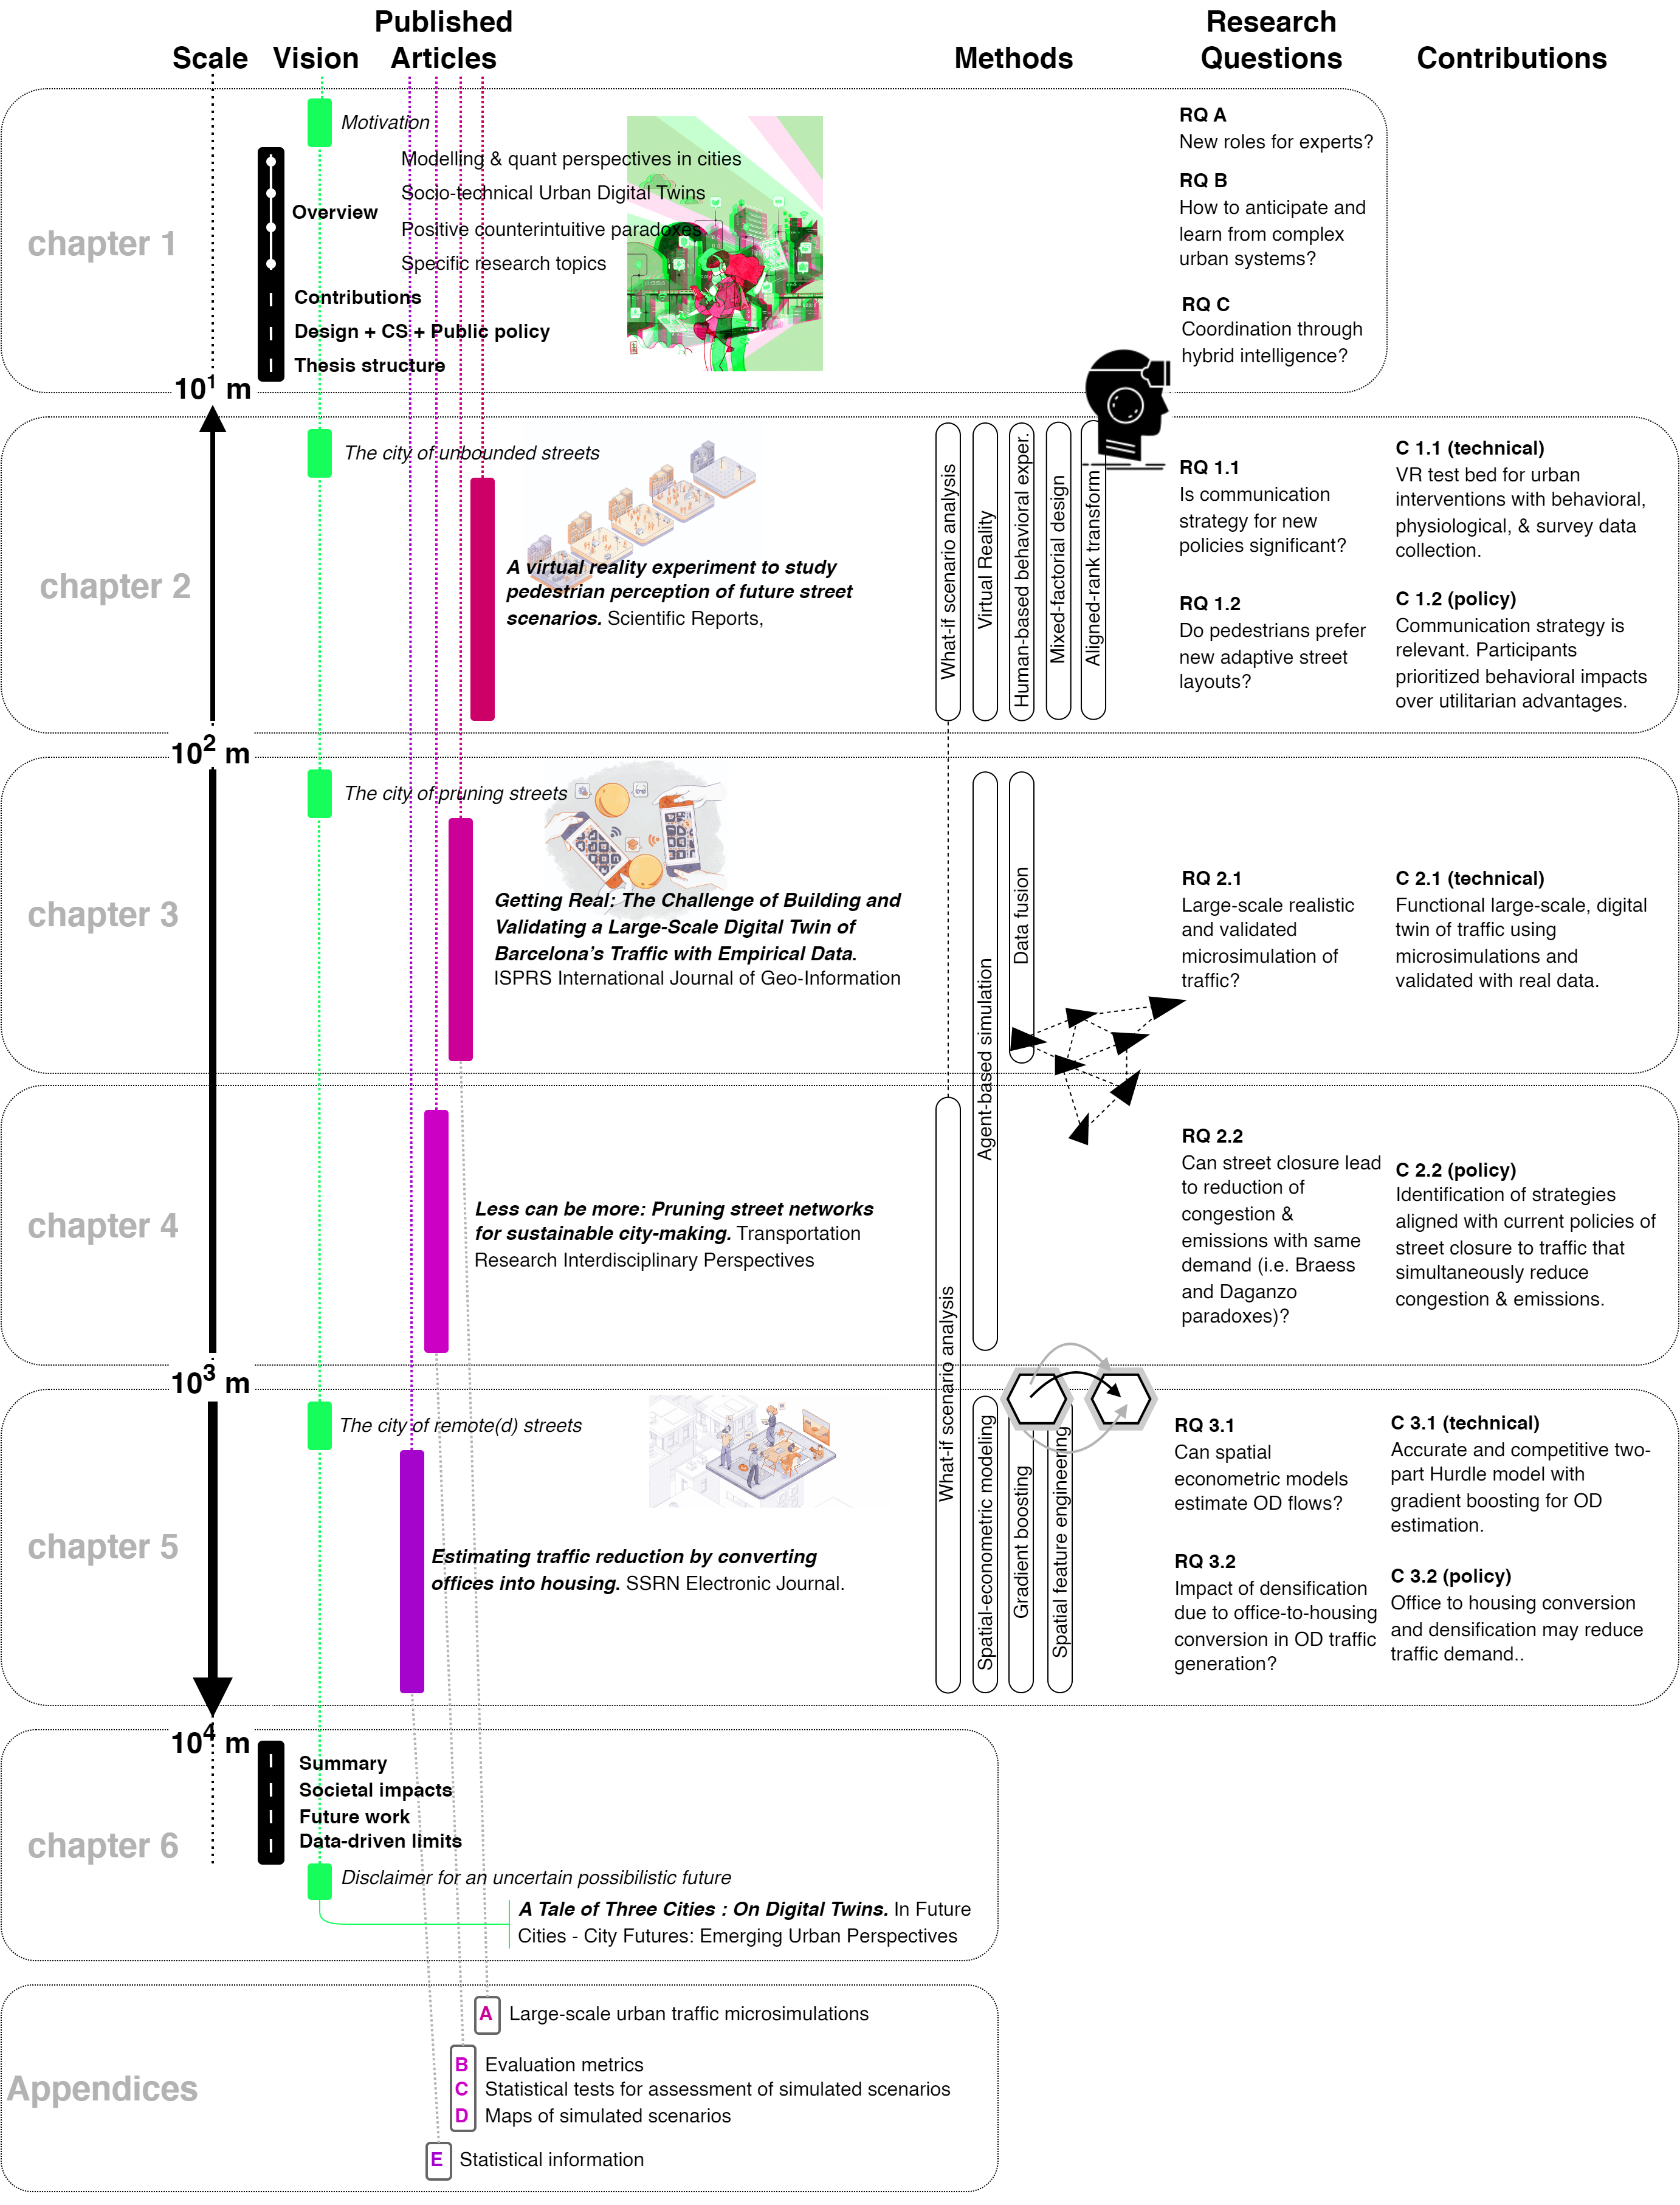
\includegraphics[width=1\textwidth]{chapters/00_introduction/figures/the_map_v04.drawio.png}
    \captionsetup{format=plain, justification=centering} % Center the caption
    \caption{Structure of the thesis, published content, research questions, and contributions in connection to the considered spatial urban scales.}
   \label{fig:thesis_map}
\end{figure}
\FloatBarrier


